\documentclass[tikz,border=10pt]{standalone}
\usetikzlibrary{calc}

\begin{document}
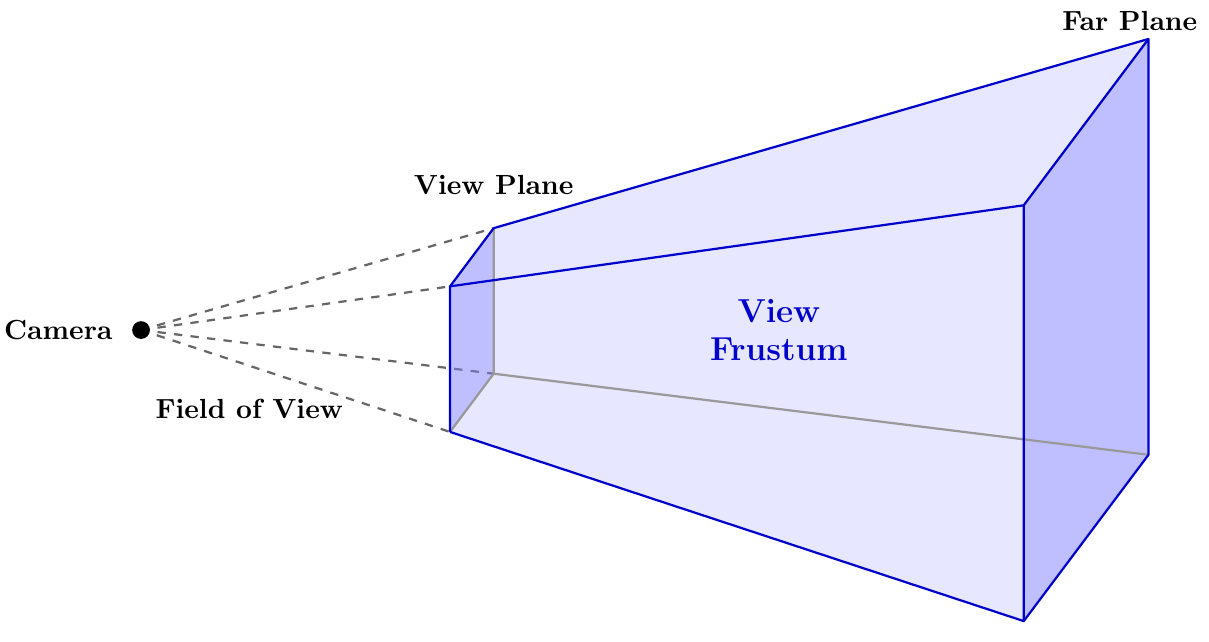
\begin{tikzpicture}[
    scale=1.2,
    line join=round,
    % Custom pseudo-3D coordinate system
    x=1cm, y=1cm, z={(-0.3cm,-0.4cm)}
]

% ---------------------------------------------------------
% 1. STRICT 2:1 BOUNDING BOX
% Width = 15, Height = 7.5 (Ratio exactly 2:1)
% Centers the diagram perfectly within these limits.
% ---------------------------------------------------------
\path [use as bounding box] (-1.2, -3) rectangle (11, 3.2);

% Define Camera (Eye)
\coordinate (C) at (0,0,0);

% Define Near Plane (View Plane) at x=3.5
\coordinate (N1) at (3.5, -0.77, -0.77); % Bottom Back (Hidden)
\coordinate (N2) at (3.5,  0.77, -0.77); % Top Back
\coordinate (N3) at (3.5,  0.77,  0.77); % Top Front
\coordinate (N4) at (3.5, -0.77,  0.77); % Bottom Front

% Define Far Plane at x=10
\coordinate (F1) at (10, -2.2, -2.2); % Bottom Back
\coordinate (F2) at (10,  2.2, -2.2); % Top Back
\coordinate (F3) at (10,  2.2,  2.2); % Top Front
\coordinate (F4) at (10, -2.2,  2.2); % Bottom Front

% Rays projecting from the camera to the near plane corners
\draw[dashed, gray!80!black, thick] (C) -- (N1);
\draw[dashed, gray!80!black, thick] (C) -- (N2);
\draw[dashed, gray!80!black, thick] (C) -- (N3);
\draw[dashed, gray!80!black, thick] (C) -- (N4);

% ---------------------------------------------------------
% 1. FILLS ONLY (Draw properties removed)
% ---------------------------------------------------------
\tikzset{frustum fill/.style={fill=blue!50, fill opacity=0.10}}
\tikzset{frustum fill bold/.style={fill=blue!50, fill opacity=0.45}}

% Fill the frustum faces (Back-to-front rendering for proper 3D transparency)
\fill[frustum fill]      (N1) -- (N2) -- (F2) -- (F1) -- cycle; % Back
\fill[frustum fill]      (N1) -- (F1) -- (F4) -- (N4) -- cycle; % Bottom
\fill[frustum fill]      (N2) -- (F2) -- (F3) -- (N3) -- cycle; % Top
\fill[frustum fill bold] (F1) -- (F2) -- (F3) -- (F4) -- cycle; % Far
\fill[frustum fill bold] (N1) -- (N2) -- (N3) -- (N4) -- cycle; % Near
\fill[frustum fill]      (N4) -- (N3) -- (F3) -- (F4) -- cycle; % Front

% ---------------------------------------------------------
% 2. LINES ONLY
% ---------------------------------------------------------
% The 3 "Hidden" lines connecting to the bottom-back corner (N1)
\draw[gray!80, thick] 
    (N4) -- (N1) -- (N2) 
    (N1) -- (F1);

% The remaining 9 visible lines mapped out in a single continuous command
\draw[blue!80!black, thick] 
    (F1) -- (F2) -- (F3) -- (F4) -- cycle  % Far plane edges
    (N2) -- (N3) -- (N4)                   % Near plane visible edges
    (N2) -- (F2)                           % Top-Back connecting edge
    (N3) -- (F3)                           % Top-Front connecting edge
    (N4) -- (F4);                          % Bottom-Front connecting edge

% Draw Camera Point
\filldraw[black] (C) circle (2.5pt);

% Labels
\node[anchor=east, font=\bfseries] at (-0.2, 0, 0) {Camera};

\node[above=0.3cm, font=\bfseries] at ($(N2)!0.0!(N3)$) {View Plane};
\node[above=0.3cm, font=\bfseries] at ($(F2)!0.15!(F3)$) {Far Plane};
\node[above=-0.8cm, font=\bfseries] at ($(C)!0.35!(N4)$) {Field of View};

\node[font=\bfseries\large, text=blue!80!black, align=center] at (6.75, 0, 0) {View\\Frustum};

\end{tikzpicture}
\end{document}